\documentclass{beamer}
\usepackage[utf8]{inputenc}
\usepackage[czech]{babel}
\usepackage{listings}
\usepackage[ruled,vlined,linesnumbered]{algorithm2e}
\usepackage{xcolor}
\usepackage{graphicx} % Přidáno pro podporu obrázků

\definecolor{codegreen}{rgb}{0,0.6,0}
\definecolor{codegray}{rgb}{0.5,0.5,0.5}
\definecolor{codepurple}{rgb}{0.58,0,0.82}
\definecolor{backcolour}{rgb}{0.95,0.95,0.92}

% Nastavení barev pro algoritmus
\SetKwComment{Comment}{/* }{ */}
\SetAlFnt{\small}
\SetAlCapFnt{\color{blue}}
\SetAlCapNameFnt{\color{blue}}
\SetKwInput{KwInput}{Input}
\SetKwInput{KwOutput}{Output}

\lstdefinestyle{mystyle}{
    backgroundcolor=\color{backcolour},   
    commentstyle=\color{codegreen},
    keywordstyle=\color{magenta},
    numberstyle=\tiny\color{codegray},
    stringstyle=\color{codepurple},
    basicstyle=\ttfamily\footnotesize,
    breakatwhitespace=false,         
    breaklines=true,                 
    captionpos=b,                    
    keepspaces=true,                 
    numbers=left,                    
    numbersep=5pt,                  
    showspaces=false,                
    showstringspaces=false,
    showtabs=false,                  
    tabsize=2
}

\lstset{style=mystyle}
\renewcommand{\algorithmcfname}{Algoritmus}
% Informace o titulní stránce
\title{TNINE - Telefonní seznam}
\author{Radim Pokorný \\ \small{xpokorr00@vutbr.cz}}
\institute{Vysoké učení technické v Brně \\ Fakulta informačních technologií}
\date{\today}

\begin{document}

\frame{\titlepage}

\begin{frame}
    \frametitle{Motivace}
    \begin{itemize}
        \item<1-> Vytvoření jednoduchého programu pro vyhledávání kontaktů
        \item<2-> Hlubší porozumnění práci s řetězci v jazyce C
        \item<3-> Zpracování telefonních čísel a jmen pomocí T9 převodu
        \item<4-> Získání zkušeností s algoritmy pro vyhledávání podřetězců
        \item<5-> Testování a ladění programu
        \item<6-> Ošetření chyb a výjimek
    \end{itemize}
\end{frame}
\begin{frame}
    \frametitle{Formulace problému}
    \begin{itemize}
        \item Cílem je vytvořit jednoduchý nástroj v jazyce C, který umožní vyhledávání kontaktů na základě uživatelského vstupu.
        \item Uživatel zadává posloupnost číslic, která se porovnává s:
        \begin{itemize}
            \item Telefonními čísly kontaktů
            \item Převedenými jmény pomocí T9 (např. „Jan“ → „526“)
        \end{itemize}
        \item Program musí efektivně zpracovávat textový vstup, vyhledávat podřetězce a vypisovat odpovídající kontakty.
        \item Důraz je kladen na správnost, robustnost a jednoduchost implementace.
    \end{itemize}
\end{frame}
\begin{frame}
    \frametitle{Schéma převodu písmen na čísla}
    \centering
    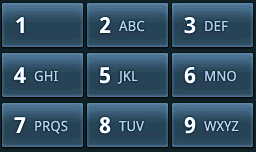
\includegraphics[height=0.2\textheight]{tnine.png} % Alternativní umístění obrázku
    \begin{itemize}
    \item a,b,c → 2
    \item d,e,f → 3
    \item g,h,i → 4
    \item j,k,l → 5
    \item m,n,o → 6
    \item p,q,r,s → 7
    \item t,u,v → 8
    \item w,x,y,z → 9
    \end{itemize}
\end{frame}

\begin{frame}
    \frametitle{Popis algoritmu}
    \begin{itemize}
    \item Algoritmus prohledává celý vstupní řetězec (telefonní číslo nebo převedené jméno).
    \item Na každé pozici kontroluje, zda od daného znaku začíná hledaný podřetězec.
    \item Pokud nalezne znak '+', nahradí ho za '0' (kvůli mezinárodním číslům).
    \item Pokud znaky odpovídají hledanému výrazu, vrátí 1 (úspěšné nalezení).
    \item Pokud podřetězec nenalezne na žádné pozici, vrací 0.
    \item Vyhledávání neodlišuje malá a velká písmena.
    \end{itemize}
\end{frame}

\begin{frame}[fragile]
\frametitle{Klíčové funkce}
\begin{itemize}
\item Převod jmen na číselné ekvivalenty
\item Podpora mezinárodních čísel (+ → 0)
\item Case-insensitive vyhledávání
\end{itemize}
\begin{algorithm}[H]
\caption{Algoritmus pro hledání podřetězce}\label{alg:one}
\For{char in \texttt{str}}{
    \If{\texttt{str[i]} je '+'}{
        \texttt{str[i]} $\gets$ '0'\Comment*[r]{Nahrazení '+' za '0'}
    }
    $j \gets 0$\;
    \While{\texttt{substr[j]} $\neq$ '\textbackslash 0' \textbf{a} \texttt{str[i+j]} $\neq$ '\textbackslash 0'}{
        \If{\texttt{str[i+j]} $\neq$ \texttt{substr[j]}}{
            \textbf{break}\Comment*[r]{Znaky se neshodují}
        }
        $j \gets j + 1$\;
    }
    \If{\texttt{substr[j]} == '\textbackslash 0'}{
        \Return{1}\Comment*[r]{Podřetězec nalezen}
    }
}
\Return{0}\Comment*[r]{Podřetězec nenalezen}
\end{algorithm}
\end{frame}

\begin{frame}[fragile]
\frametitle{Příklad použití}
\begin{exampleblock}{Vstup}
\begin{lstlisting}[basicstyle=\ttfamily\small]
Jan
+420123456789
Petr
555-987654
Anna
123456
\end{lstlisting}
\end{exampleblock}

\begin{block}{Výstup pro hledání "56"}
\begin{lstlisting}[basicstyle=\ttfamily\small]
jan, +420123456789
anna, 123456
\end{lstlisting}
\end{block}

\begin{alertblock}{Poznámka}
Program podporuje jak vyhledávání v číslech, tak převod jmen na T9 číselnou reprezentaci
\end{alertblock}
\end{frame}

\begin{frame}
\frametitle{Ošetření chyb při testování}
\begin{itemize}
\item Kontrola platnosti vstupního argumentu (pouze čísla)
\item Omezení délky vstupu (max 100 znaků)
\item Omezení počtu kontaktů (max 100)
\item Zacházení se speciálními znaky (+, -)
\item Vypsání "Not found" při nenalezení shody
\end{itemize}
\end{frame}
\begin{frame}
    \frametitle{Vyhodnocení implementace}
    \begin{itemize}
        \item Program byl otestován na různých vstupech – jak validních, tak chybných.
        \item Funguje jak pro mezinárodní, tak běžná telefonní čísla (včetně znaků jako '+' nebo '-').
        \item Podporuje vyhledávání v jménech i číslech, bez ohledu na velikost písmen.
        \item Překlad jmen do T9 je implementován jednoduše, ale efektivně.
        \item Implementace je vhodná pro menší vstupy (do 100 kontaktů), při větších objemech by bylo vhodné optimalizovat např. použitím tries a ukazatelů.
    \end{itemize}
\end{frame}
\begin{frame}
\frametitle{Závěr}
\begin{columns}
\begin{column}{0.7\textwidth}
\begin{itemize}
\item Jednoduchý, ale praktický nástroj
\item Demonstrace práce s řetězci v jazyce C
\item Možnosti rozšíření:
\begin{itemize}
\item Grafické rozhraní
\item Podpora více znakových sad
\item Optimalizace pro velké databáze
\end{itemize}
\end{itemize}
\end{column}
\begin{column}{0.3\textwidth}
\end{column}
\end{columns}

\vspace{0.5cm}
\centering
\Large{Děkuji za pozornost!}
\end{frame}

\end{document}